%%%%%%%%%%%%%%%%%%%%%%%%%%%%%%%%%%%%%%%%%%%%%%%%%%%%%%%%%%%%%%%%%%%%%%%%%%%%%%%%
% Présentation : Introduction à Git
% Thème : Formation Club (Beamer avec Miniframes & CambridgeUS)
% Licence : CC BY-NC-SA 4.0
%%%%%%%%%%%%%%%%%%%%%%%%%%%%%%%%%%%%%%%%%%%%%%%%%%%%%%%%%%%%%%%%%%%%%%%%%%%%%%%%

\documentclass[
	11pt,
	aspectratio=169
]{beamer}


%----------------------------------------------------------------------------------------
%	PACKAGES ET CONFIGURATION LINGUISTIQUE
%----------------------------------------------------------------------------------------
\usepackage[utf8]{inputenc}
\usepackage[T1]{fontenc}
\usepackage[french]{babel}
\usepackage{booktabs}
\usepackage{tikz}
\usetikzlibrary{arrows.meta, positioning, shapes.geometric, backgrounds, fit}
\usepackage{listings}
\usepackage{ccicons} % Icônes Creative Commons
\usepackage{ulem}

%----------------------------------------------------------------------------------------
%	SÉLECTION DU THÈME ET POLICES
%----------------------------------------------------------------------------------------
\usetheme{CambridgeUS}
\useinnertheme{circles}
\useoutertheme{miniframes} % Active les points de navigation en haut

\usepackage[default]{opensans}

% Palette Git personnalisée
\definecolor{gitred}{RGB}{240, 80, 50}      % Orange-Rouge Git officiel
\definecolor{gitdark}{RGB}{36, 41, 46}      % Gris ardoise GitHub
\definecolor{gitlight}{RGB}{246, 248, 250}  % Gris clair de fond
\definecolor{gitblue}{RGB}{3, 102, 214}     % Bleu Git
\definecolor{gitgreen}{RGB}{40, 167, 69}    % Vert succès
\definecolor{gitborder}{RGB}{209, 213, 218} % Bordure neutre

% Application des couleurs
% \setbeamercolor{palette primary}{bg=gitdark, fg=white}
% \setbeamercolor{palette secondary}{bg=gitred!90!black, fg=white}
% \setbeamercolor{palette tertiary}{bg=gitred, fg=white}
% \setbeamercolor{structure}{fg=gitred}
% \setbeamercolor{titlelike}{parent=palette primary, fg=gitred}
% \setbeamercolor{frametitle}{bg=gitdark, fg=white}
% \setbeamercolor{mini frame}{fg=gitred}
% \setbeamercolor{section in head/foot}{bg=gitdark, fg=white}
% \setbeamercolor{block title}{bg=gitred, fg=white}
% \setbeamercolor{block body}{bg=gitlight, fg=black}
% \setbeamercolor{block title example}{bg=gitdark, fg=white}
% \setbeamercolor{block body example}{bg=gitlight, fg=black}

% Rétablissement du pied de page infolines avec les miniframes en haut
\makeatletter
\setbeamertemplate{footline}{
  \leavevmode%
  \hbox{%
  \begin{beamercolorbox}[wd=.333333\paperwidth,ht=2.25ex,dp=1ex,center]{author in head/foot}%
    \usebeamerfont{author in head/foot}\insertshortauthor
  \end{beamercolorbox}%
  \begin{beamercolorbox}[wd=.333333\paperwidth,ht=2.25ex,dp=1ex,center]{title in head/foot}%
    \usebeamerfont{title in head/foot}\insertshorttitle
  \end{beamercolorbox}%
  \begin{beamercolorbox}[wd=.333333\paperwidth,ht=2.25ex,dp=1ex,right]{date in head/foot}%
    \usebeamerfont{date in head/foot}\insertshortdate{}\hspace*{1.5em}
    \insertframenumber{} / \inserttotalframenumber\hspace*{1.5ex}
  \end{beamercolorbox}}%
  \vskip0pt%
}
\makeatother

% Symbole d'interdiction vectoriel compatible pdflatex / latexmk
\newcommand{\noban}{%
    \tikz[baseline=-0.6ex]{%
        \draw[red, line width=1.2pt] (0,0) circle (0.9ex);%
        \draw[red, line width=1.2pt] (-0.63ex, 0.63ex) -- (0.63ex, -0.63ex);%
    }%
}

%----------------------------------------------------------------------------------------
%	CONFIGURATION LISTINGS (CORRECTION DES ACCENTS UTF-8)
%----------------------------------------------------------------------------------------
\lstdefinestyle{gitstyle}{
    basicstyle=\ttfamily\footnotesize,
    backgroundcolor=\color{gitlight},
    frame=single,
    rulecolor=\color{gitborder},
    keywordstyle=\color{gitred}\bfseries,
    commentstyle=\color{gray}\itshape,
    stringstyle=\color{gitblue},
    breaklines=true,
    showstringspaces=false,
    inputencoding=utf8,
    extendedchars=true,
    literate=
        {á}{{\'a}}1 {é}{{\'e}}1 {í}{{\'i}}1 {ó}{{\'o}}1 {ú}{{\'u}}1
        {Á}{{\'A}}1 {É}{{\'E}}1 {Í}{{\'I}}1 {Ó}{{\'O}}1 {Ú}{{\'U}}1
        {à}{{\`a}}1 {è}{{\`e}}1 {ì}{{\`i}}1 {ò}{{\`o}}1 {ù}{{\`u}}1
        {À}{{\`A}}1 {È}{{\`E}}1 {Ì}{{\`I}}1 {Ò}{{\`O}}1 {Ù}{{\`U}}1
        {ä}{{\"a}}1 {ë}{{\"e}}1 {ï}{{\"i}}1 {ö}{{\"o}}1 {ü}{{\"u}}1
        {Ä}{{\"A}}1 {Ë}{{\"E}}1 {Ï}{{\"I}}1 {Ö}{{\"O}}1 {Ü}{{\"U}}1
        {â}{{\^a}}1 {ê}{{\^e}}1 {î}{{\^i}}1 {ô}{{\^o}}1 {û}{{\^u}}1
        {Â}{{\^A}}1 {Ê}{{\^E}}1 {Î}{{\^I}}1 {Ô}{{\^O}}1 {Û}{{\^U}}1
        {œ}{{\oe}}1 {Œ}{{\OE}}1 {æ}{{\ae}}1 {Æ}{{\AE}}1
        {ç}{{\c{c}}}1 {Ç}{{\c{C}}}1
        {«}{{\og}}1 {»}{{\fg}}1
}
\lstset{style=gitstyle}

%----------------------------------------------------------------------------------------
%	MÉTADONNÉES DE LA PRÉSENTATION
%----------------------------------------------------------------------------------------
\title[Introduction à Git]{Introduction à Git}
\subtitle{Formation Robotech}
\author[Timothée pour Robotech]{Timothée}
\institute[Robotech]{\url{https://github.com/Robotech-Lillois}}
\date[\today \quad \ccbyncsa]{\today}

% Logo sur la première page
\titlegraphic{
    \vspace{-0.5cm}
    \IfFileExists{./img/logo.png}{%
        
\includegraphics[height=1.4cm,keepaspectratio]{./img/logo.png}%
    }{%
        \fbox{\color{gitdark}\small\strut Emplacement ./img/logo.png}%
    }
}

\setbeamertemplate{headline}{%
    \leavevmode%
    \begin{beamercolorbox}[wd=\paperwidth,ht=2.5ex,dp=3.0ex]{section in head/foot}%
        % 1. Navigation dots restricted to the left
        \insertnavigation{\dimexpr\paperwidth - 1.5cm\relax}%
        \hfill%
        % 2. Logo on the right with vertical centering and right margin
        \IfFileExists{./img/logo.png}{%
            \raisebox{-2.5ex}{
\includegraphics[height=4.5ex,keepaspectratio]{./img/logo.png}}%
        }{%
            \fbox{\tiny .\/img\/logo}%
        }%
        \hspace*{0.4cm}% Right margin from the slide edge
    \end{beamercolorbox}%
}

% Compteur automatique pour animation multi-frames
\newcounter{animstep}
\makeatletter
\newcommand{\startanim}[1]{%
    \setcounter{animstep}{0}%
    \def\currentanimname{#1}%
}
\newcommand{\stepanim}{%
    \stepcounter{animstep}%
    (\theanimstep/\ref*{\currentanimname})%
}
\newcommand{\stopanim}{%
    % Force le label à enregistrer la valeur de animstep et non le numéro de slide Beamer
    \edef\@currentlabel{\the\value{animstep}}%
    \label{\currentanimname}%
}
\makeatother


%----------------------------------------------------------------------------------------
%	DÉBUT DU DOCUMENT
%----------------------------------------------------------------------------------------
\begin{document}

%========================================================================================
% SLIDE 1 : TITRE
%========================================================================================
\begin{frame}
    \titlepage
    \vspace{-0.6cm}
    \begin{center}
        \footnotesize
        \ccbyncsa\ Ce support est mis à disposition sous licence \textbf{CC BY-NC-SA 4.0}
    \end{center}
\end{frame}

%========================================================================================
% SLIDE 2 : SOMMAIRE
%========================================================================================
\begin{frame}
    \frametitle{Sommaire}
    \tableofcontents
\end{frame}

%========================================================================================
\section{Introduction}
%========================================================================================
% \subsection{Qu'est-ce que Git ?}

\begin{frame}
    \frametitle{Qu'est-ce que Git ?}
    \begin{itemize}
        \item \textbf{Un gestionnaire de versions} :
        \begin{itemize}
            \item Conçu en 2005 par \textit{Linus Torvalds} pour gérer du code
            \item Sauvegarde toutes les modifications
        \end{itemize}
        \bigskip
        \item \textbf{Un outil de travail collaboratif} :
        \begin{itemize}
            \item Facilite le partage de code
            \item Permet de travailler en même temps sur un même projet
        \end{itemize}
        \bigskip
        \item \textbf{Un outil efficace et rapide} :
        \begin{itemize}
            \item Conçu initialement pour le kernel Linux
            \item Fait pour être utilisé par de grands projets
        \end{itemize}
    \end{itemize}
\end{frame}

% \subsection{Pourquoi Git ?}
\begin{frame}
    \frametitle{Pourquoi Git ?}
        \begin{itemize}
            \item \textbf{Des dizaines de versions dans un seul fichier} : \sout{projet\_final.odt, projet\_v2\_final\_final5.odt}, \dots  $\Rightarrow$ \textbf{projet.odt}
            \item \textbf{Droit à l'erreur} : Possibilité d'inspecter ou d'annuler n'importe quelle modification passée
            \item \textbf{Travail collaboratif plus simple} : Plusieurs personnes peuvent coder simultanément sans écraser le code ddes autres
            \item \textbf{Branches indépendantes} : Tester des fonctionnalités sans casser les autres versions
            \item \textbf{Standard universel} du monde pro ET de la recherche.
        \end{itemize}
\end{frame}

% \subsection{Git vs GitHub}
\begin{frame}
    \frametitle{Git vs GitHub}
    \framesubtitle{outil local VS service d'hébergement}

    \begin{columns}[t]
        \begin{column}{0.48\textwidth}
            \begin{block}{\centering \textbf{Git (outil local)}}
                \begin{itemize}
                    \item Logiciel en ligne de commande (CLI)
                    \item 100\% autonome sans accès Internet
                    \item open-source
                    \item Crée les commits, gère les branches et les fusions
                \end{itemize}
            \end{block}
        \end{column}

        \begin{column}{0.48\textwidth}
            \begin{exampleblock}{\centering \textbf{GitHub / GitLab / Gitea (Plateforme Web)}}
                \begin{itemize}
                    \item Serveur d'hébergement distant
                    \item Interface graphique et exploration web
                    \item Autres outils : Pull Requests, ...
                \end{itemize}
            \end{exampleblock}
        \end{column}
    \end{columns}
\end{frame}

%========================================================================================
\section{Philosophie}
%========================================================================================
% \subsection{Les 4 zones de Git}

%========================================================================================
% SLIDE : Le Workflow Git (Explication basée sur l'image)
%========================================================================================
\begin{frame}
    \frametitle{Le Workflow Git}
    \centering
    \IfFileExists{./img/workflow.png}{%
        \vspace{-0.0cm}
        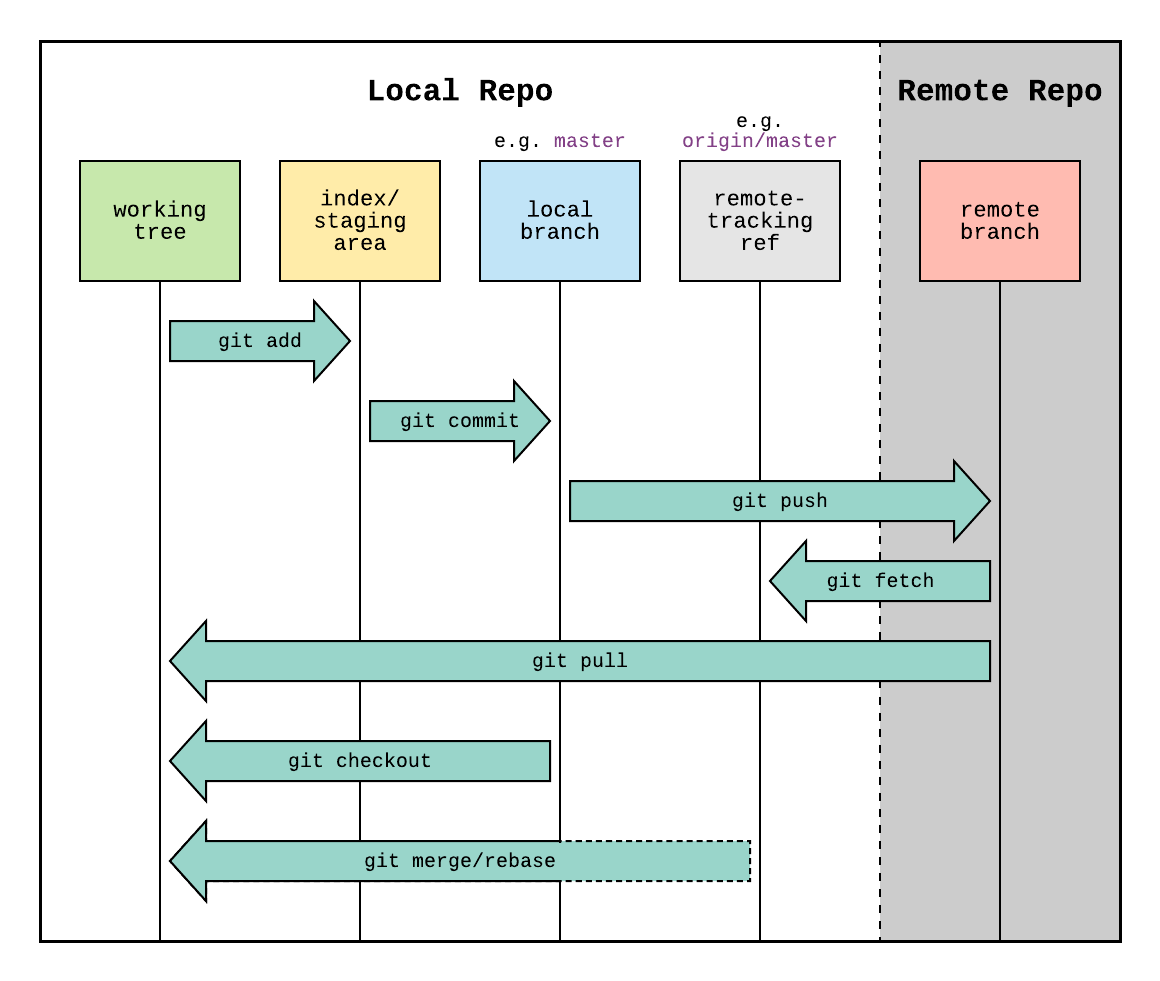
\includegraphics[height=0.9\textheight,keepaspectratio]{./img/workflow.png}%
    }{%
        \fbox{\begin{minipage}[c]{0.95\linewidth}\centering Image \texttt{./img/workflow.png} manquante\end{minipage}}%
    }
\end{frame}

%========================================================================================
% SLIDE : Explication du Git Flow
%========================================================================================
\begin{frame}
    \frametitle{Git Flow}

    \begin{center}
        \IfFileExists{./img/gitflow.png}{%
            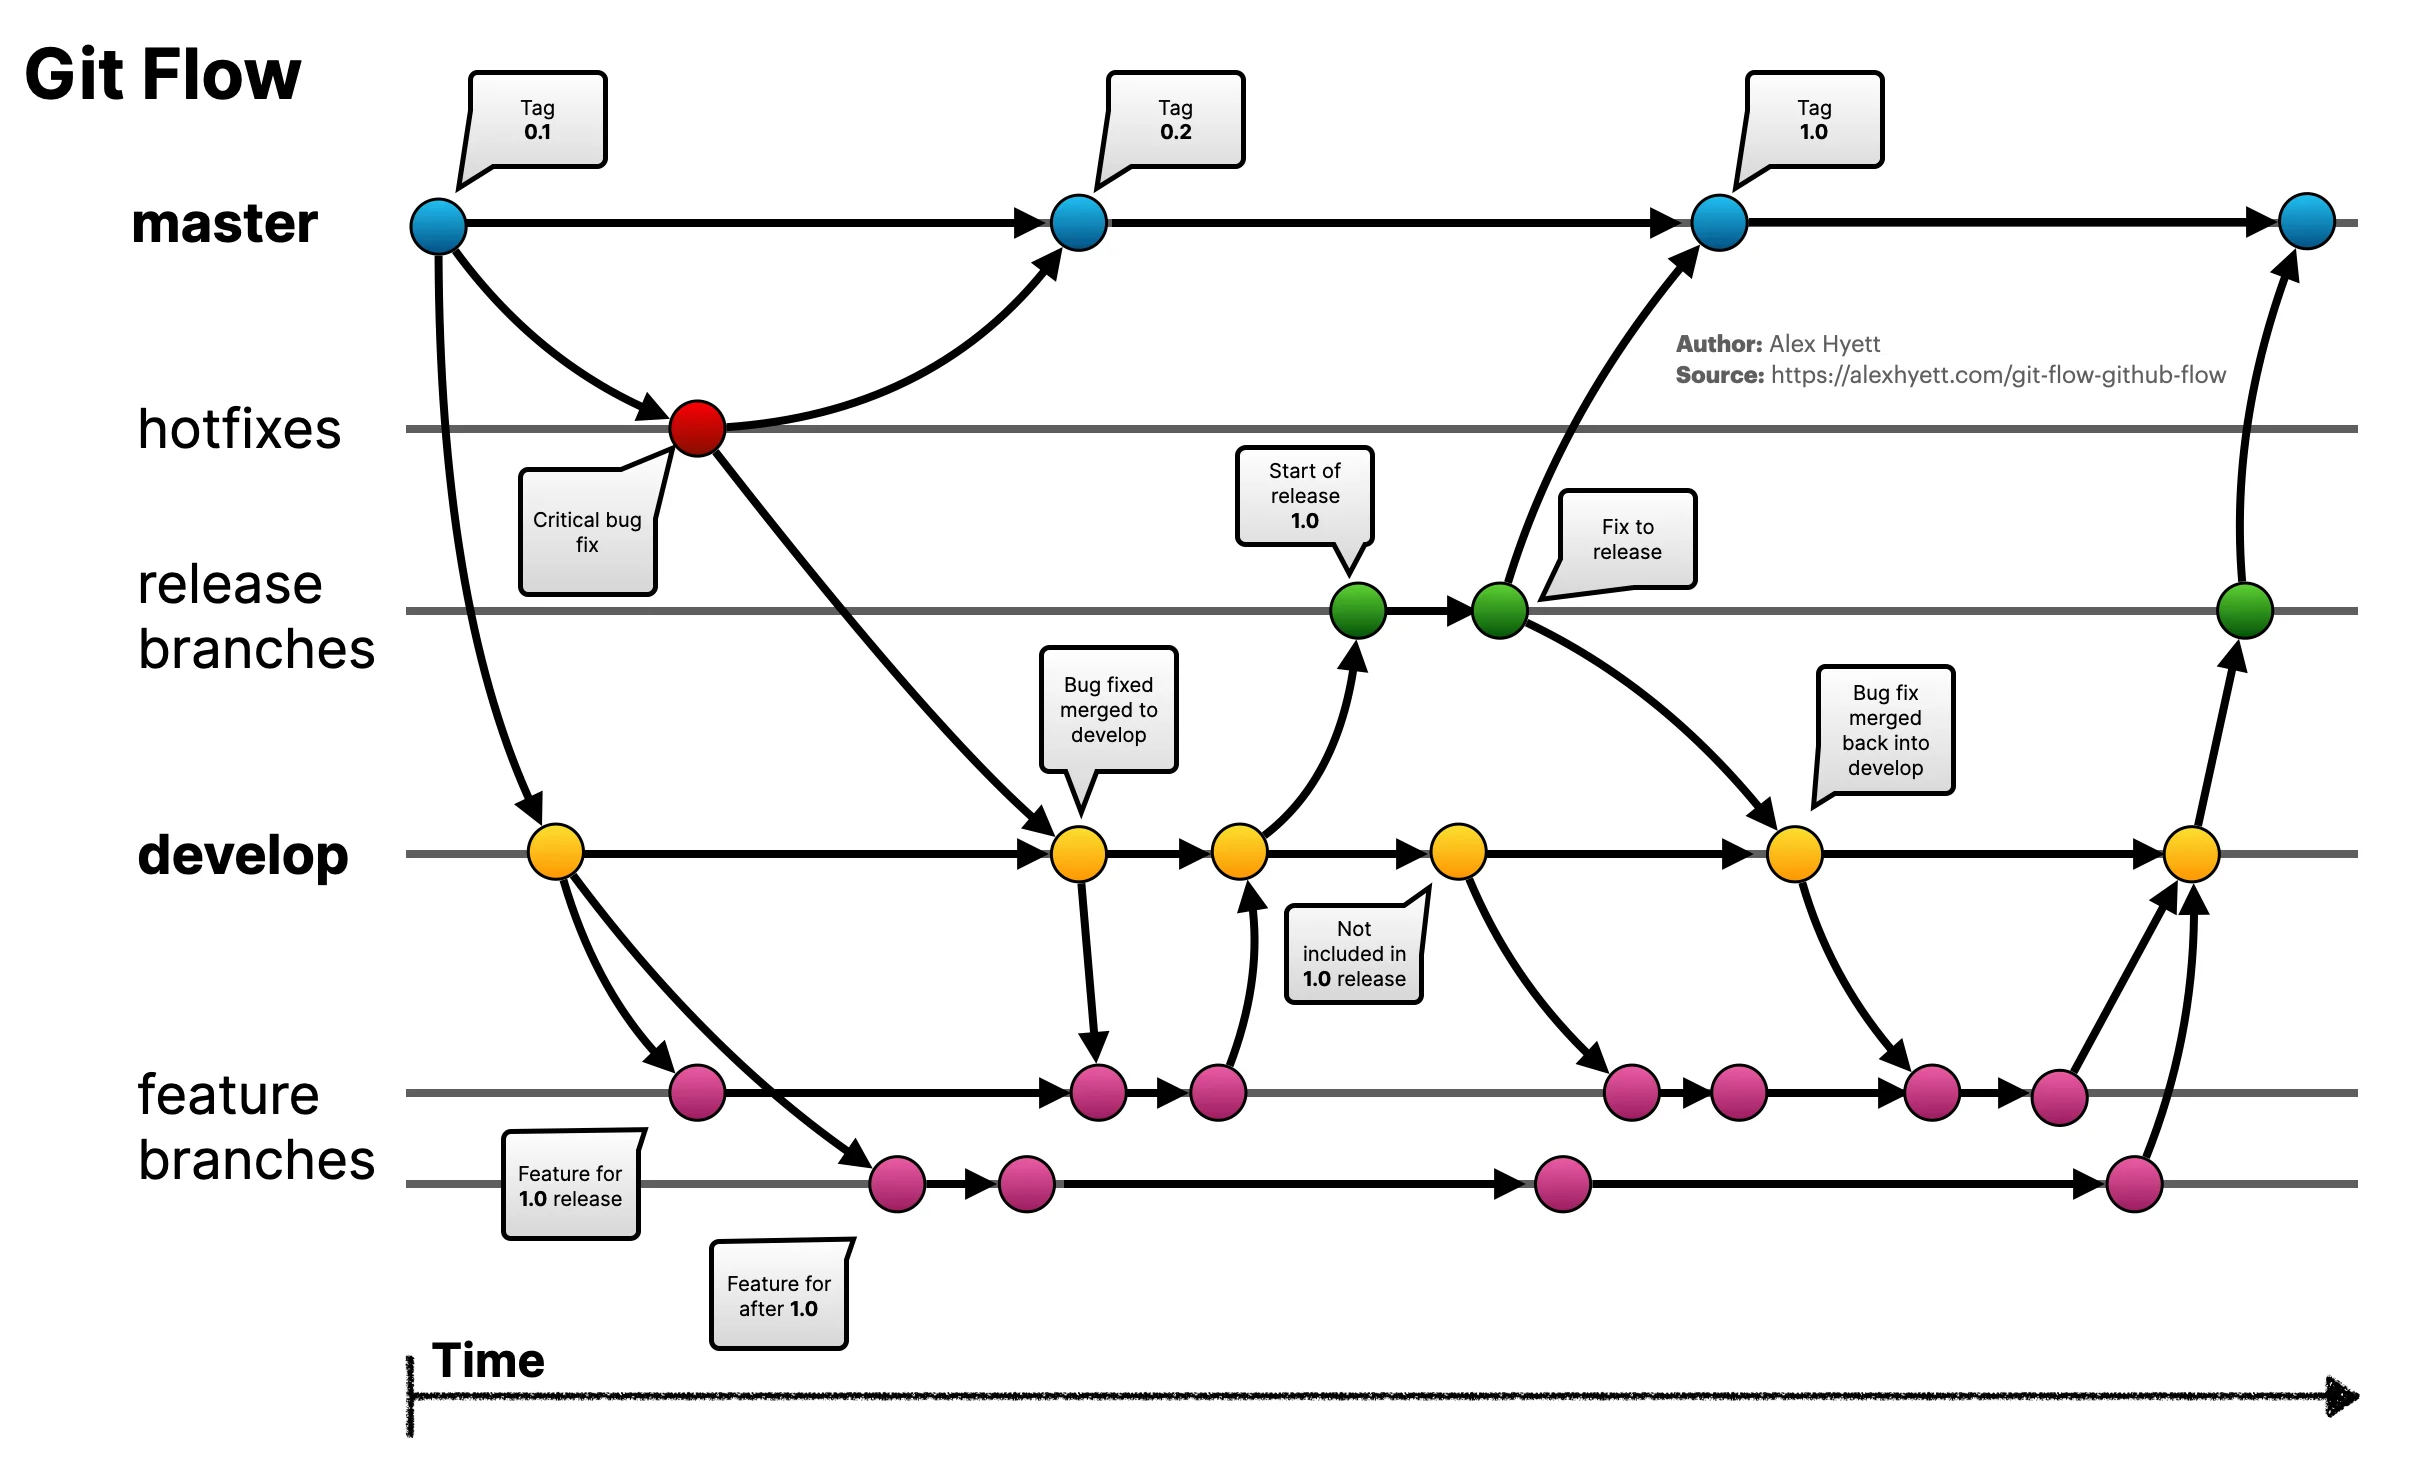
\includegraphics[height=7cm,keepaspectratio]{./img/gitflow.png}%
        }{%
            \fbox{\begin{minipage}[c][3.8cm][c]{0.95\linewidth}\centering Image \texttt{./img/gitflow.png} manquante\end{minipage}}%
        }
    \end{center}
\end{frame}

% \subsection{Branches \& Fusion}


% \subsection{Cycle local \& Inspection}

\section{Les bases}
\begin{frame}[fragile]
    \frametitle{Commandes de base}
    \framesubtitle{initialiser - préparer - enregistrer}

    \begin{enumerate}
        \item \textbf{\texttt{git init}} : Initialise un dépôt local dans le dossier courant (crée \texttt{.git/}).
\begin{lstlisting}[language=bash]
git init
\end{lstlisting}

        \item \textbf{\texttt{git add}} : Ajoute des fichiers modifiés à l'index (\textit{staging area}).
\begin{lstlisting}[language=bash]
git add main.py         # Ajoute un fichier précis
git add .               # Prépare l'ensemble des fichiers modifiés
\end{lstlisting}

        \item \textbf{\texttt{git commit}} : Enregistre le commit avec un message \textbf{explicite !}
\begin{lstlisting}[language=bash]
git commit -m "feature: ajout de la fonction add_vectors dans math.h"
\end{lstlisting}
    \end{enumerate}
\end{frame}

\begin{frame}[fragile]
    \frametitle{Commandes de base}
    \framesubtitle{Connaître l'état du projet}

    \begin{enumerate}
        \item \textbf{\texttt{git status}} : Présente l'état des fichiers (modifiés, suivis, indexés).
\begin{lstlisting}[language=bash]
git status
\end{lstlisting}

        \item \textbf{\texttt{git diff}} : Affiche les écarts exacts de code ligne par ligne.
\begin{lstlisting}[language=bash]
git diff                # Modifications non indexées
git diff --staged       # Modifications prêtes pour le prochain commit
\end{lstlisting}

        \item \textbf{\texttt{git log}} : Visualise l'historique chronologique des commits.
\begin{lstlisting}[language=bash]
git log --oneline --graph --all
\end{lstlisting}
    \end{enumerate}
\end{frame}

% \subsection{Synchronisation \& .gitignore}

\begin{frame}[fragile]
    \frametitle{Commandes de base}
    \framesubtitle{Synchronisation distante}

    \begin{enumerate}
        \item \textbf{\texttt{git clone}} : Télécharge une copie intégrale d'un dépôt distant existant.
\begin{lstlisting}[language=bash]
git clone https://github.com/Robotech-Lillois/Chessboard.git
\end{lstlisting}

        \item \textbf{\texttt{git remote}} : Ajoute un repo distant comme source
\begin{lstlisting}
git remote add origin https://github.com/Robotech-Lillois/Formation
\end{lstlisting}

        \item \textbf{\texttt{git pull}} : Récupère et fusionne les commits distants sur votre branche locale.
\begin{lstlisting}[language=bash]
git pull origin main
\end{lstlisting}

        \item \textbf{\texttt{git push}} : Publie vos commits locaux validés vers le serveur distant.
\begin{lstlisting}[language=bash]
git push origin main
\end{lstlisting}
    \end{enumerate}
\end{frame}

\begin{frame}[fragile]
    \frametitle{Le fichier \texttt{.gitignore}}
    \framesubtitle{Exclure certains fichiers}

    \begin{itemize}
        \item Fichier placé à la racine du dépôt indiquant les motifs à ne jamais indexer.
        \item Indispensable pour garder un dépôt clair et ne pas faire fuiter certaines infos.
    \end{itemize}

    \begin{exampleblock}{Exemple de fichier \texttt{.gitignore}}
\begin{lstlisting}
# Fichiers sensibles (JAMAIS sur un dépôt Git !)
mot-de-passe.txt

# Dépendances et fichiers générés
__pycache__/
*.o
*.pdf

# Fichiers temporaires des systèmes d'exploitation
.DS_Store
Thumbs.db
\end{lstlisting}
    \end{exampleblock}
\end{frame}

%========================================================================================
% SLIDE : L'IMPORTANCE DU README.MD
%========================================================================================
\begin{frame}
    \frametitle{Le \texttt{README.md}}
    \framesubtitle{Un fichier à ne pas négliger}

    \begin{columns}[t]
        % Colonne 1 : Rôle et importance
        \begin{column}{0.48\textwidth}
            \begin{block}{\footnotesize Pourquoi est-il indispensable ?}
                \scriptsize
                \begin{itemize}
                    \item \textbf{1ère impression} : 1er fichier lu et affiché par défaut sur GitHub / GitLab
                    \item \textbf{Autonomie} : permet à un arrivant d'installer et tester le projet sans vous solliciter
                    \item \textbf{Format Markdown} : simple en texte brut, riche à l'affichage web
                \end{itemize}
            \end{block}

            \vskip 2pt
            \begin{alertblock}{\centering \scriptsize Règle d'or}
                \centering \scriptsize
                Un code sans \texttt{README} est un inutilisable pour les autres
            \end{alertblock}
        \end{column}

        % Colonne 2 : Structure minimale
        \begin{column}{0.48\textwidth}
            \begin{exampleblock}{\footnotesize Structure minimale en 5 points}
                \scriptsize
                \begin{enumerate}
                    \item \textbf{Titre \& Pitch} : nom du projet et rôle en 1 phrase.
                    \item \textbf{Installation} : dépendances et commandes de setup.
                    \item \textbf{Usage} : exemple minimal pour lancer le code.
                    \item \textbf{Contribution} : consignes pour soumettre une PR.
                    \item \textbf{Licence} : conditions légales d'utilisation (MIT, GPL...).
                \end{enumerate}
            \end{exampleblock}
        \end{column}
    \end{columns}
\end{frame}

\section{Branches}
%========================================================================================
% SLIDE : Commandes complètes de branches
%========================================================================================

\begin{frame}[fragile]
    \frametitle{Les Branches}
    \framesubtitle{Ne pas travailler sur le main !}

    \begin{center}
    \begin{tikzpicture}[
        commit/.style={circle, draw=gitdark, fill=gitlight, thick, minimum size=0.65cm, inner sep=0pt, font=\scriptsize\bfseries},
        branch/.style={rectangle, rounded corners=3pt, fill=gitred, text=white, font=\tiny\bfseries, inner sep=3pt},
        mainb/.style={rectangle, rounded corners=3pt, fill=gitdark, text=white, font=\tiny\bfseries, inner sep=3pt},
        arr/.style={->, >=stealth, thick}
    ]
        % Commits sur main
        \node[commit] (c1) {C1};
        \node[commit, right=0.9cm of c1] (c2) {C2};
        \node[commit, right=1.8cm of c2] (c3) {C3};
        \node[mainb, right=0.3cm of c3] (bmain) {main};

        % Commits sur feature
        \node[commit, above right=0.55cm and 0.8cm of c2, fill=gitred!20, draw=gitred] (c4) {C4};
        \node[commit, right=0.9cm of c4, fill=gitred!20, draw=gitred] (c5) {C5};
        \node[branch, right=0.3cm of c5] (bfeat) {feature};
        \node[rectangle, draw=gitred, dashed, fill=white, font=\tiny\bfseries, above=0.2cm of bfeat] (head) {HEAD};

        % Liens
        \draw[arr] (c1) -- (c2);
        \draw[arr] (c2) -- (c3);
        \draw[arr] (c3) -- (bmain);
        \draw[arr, gitred] (c2) |- (c4);
        \draw[arr, gitred] (c4) -- (c5);
        \draw[arr, gitred] (c5) -- (bfeat);
        \draw[arr, gitred] (head) -- (bfeat);
    \end{tikzpicture}
    \end{center}

    \begin{block}{Commandes principales}
\begin{lstlisting}[language=bash]
git switch -c feature-strophe   # Crée et bascule sur la branche feature
git branch -v                   # Liste toutes les branches locales
git switch main                 # Revient sur la branche principale
\end{lstlisting}
    \end{block}
\end{frame}

%========================================================================================
% SLIDE : LES 3 STRATÉGIES DE FUSION (DÉTAILLÉ & ÉQUILIBRÉ)
%========================================================================================
\begin{frame}
    \frametitle{Le Merge}
    \framesubtitle{Comparaison des options \texttt{--ff}, \texttt{--no-ff} et \texttt{--ff-only}}

    % Styles TikZ compacts
    \tikzset{
        mDot/.style={circle, draw=gitdark, fill=gitlight, thick, minimum size=0.42cm, inner sep=0pt, font=\fontsize{5}{6}\selectfont\bfseries},
        mFeat/.style={circle, draw=gitred, fill=gitred!20, thick, minimum size=0.42cm, inner sep=0pt, font=\fontsize{5}{6}\selectfont\bfseries},
        mMerge/.style={circle, draw=gitgreen, fill=gitgreen!25, thick, minimum size=0.42cm, inner sep=0pt, font=\fontsize{5}{6}\selectfont\bfseries},
        mTag/.style={rectangle, rounded corners=2pt, font=\fontsize{4.5}{5.5}\selectfont\bfseries, inner sep=1.5pt},
        mArr/.style={->, >=stealth, semithick}
    }

    \begin{columns}[t]
        %--------------------------------------------------------------------------------
        % COLONNE 1 : --ff
        %--------------------------------------------------------------------------------
        \begin{column}{0.32\textwidth}
            \begin{block}{\centering \footnotesize \texttt{--ff} (Défaut)}
                \centering
                \begin{tikzpicture}[baseline=(c1.base)]
                    \path (-0.2, -0.55) rectangle (2.6, 0.55);
                    \node[mDot] (c1) at (0, 0) {C1};
                    \node[mDot] (c2) at (0.6, 0) {C2};
                    \node[mFeat] (c3) at (1.2, 0) {C3};
                    \node[mFeat] (c4) at (1.8, 0) {C4};
                    \draw[mArr] (c1) -- (c2);
                    \draw[mArr, gitred] (c2) -- (c3);
                    \draw[mArr, gitred] (c3) -- (c4);
                    \node[mTag, fill=gitdark, text=white, below=0.08cm of c4] {main};
                \end{tikzpicture}

                \vskip 2pt
                \scriptsize
                \begin{itemize}
                    \item Avance simple du pointeur
                    \item Zéro commit créé si ligne droite
                    \item Divergence $\Rightarrow$ 3-way merge auto
                    \item Risque : crée des commits de fusion involontaires lors d'un \texttt{pull}
                \end{itemize}
            \end{block}
        \end{column}

        %--------------------------------------------------------------------------------
        % COLONNE 2 : --no-ff
        %--------------------------------------------------------------------------------
        \begin{column}{0.32\textwidth}
            \begin{exampleblock}{\centering \footnotesize \texttt{--no-ff}}
                \centering
                \begin{tikzpicture}[baseline=(c1.base)]
                    \path (-0.2, -0.55) rectangle (2.6, 0.55);
                    \node[mDot] (c1) at (0, 0) {C1};
                    \node[mDot] (c2) at (0.6, 0) {C2};
                    \node[mFeat] (c3) at (1.1, 0.32) {C3};
                    \node[mFeat] (c4) at (1.7, 0.32) {C4};
                    \node[mMerge] (m) at (2.3, 0) {M};
                    \draw[mArr] (c1) -- (c2);
                    \draw[mArr, gitred] (c2) |- (c3);
                    \draw[mArr, gitred] (c3) -- (c4);
                    \draw[mArr] (c2) -- (m);
                    \draw[mArr, gitred] (c4) -| (m);
                    \node[mTag, fill=gitdark, text=white, below=0.08cm of m] {main};
                \end{tikzpicture}

                \vskip 2pt
                \scriptsize
                \begin{itemize}
                    \item Commit de fusion \textbf{M} forcé
                    \item Isole et groupe la fonctionnalité
                    \item Facilite l'annulation complète d'une feature (\texttt{revert} en 1 commit)
                    \item Recommandé pour les \textit{Pull Requests}
                \end{itemize}
            \end{exampleblock}
        \end{column}

        %--------------------------------------------------------------------------------
        % COLONNE 3 : --ff-only
        %--------------------------------------------------------------------------------
        \begin{column}{0.32\textwidth}
            \begin{alertblock}{\centering \footnotesize \texttt{--ff-only}}
                \centering
                \begin{tikzpicture}[baseline=(c1.base)]
                    \path (-0.2, -0.55) rectangle (2.6, 0.55);
                    \node[mDot] (c1) at (0, 0) {C1};
                    \node[mDot] (c2) at (0.6, 0) {C2};
                    \node[mDot] (c5) at (1.2, 0.32) {C5};
                    \node[mFeat] (c3) at (1.2, -0.32) {C3};
                    \draw[mArr] (c1) -- (c2);
                    \draw[mArr] (c2) |- (c5);
                    \draw[mArr, gitred] (c2) |- (c3);
                    \node[font=\fontsize{5}{6}\selectfont\bfseries, red] at (2.0, 0) {\texttimes\ REFUS};
                \end{tikzpicture}

                \vskip 2pt
                \scriptsize
                \begin{itemize}
                    \item Avance rapide obligatoire
                    \item Divergence $\Rightarrow$ Arrêt net (\textit{abort})
                    \item Zéro fichier pollué par un conflit
                    \item Impose un \texttt{rebase} préalable (garantit un historique 100\% plat)
                \end{itemize}
            \end{alertblock}
        \end{column}
    \end{columns}
    \center\scriptsize\textit{Note : ff = fast forward}
\end{frame}

%========================================================================================
% ANIMATION : WORKFLOW AVEC --FF-ONLY ET RÉSOLUTION PAR REBASE (6 ÉTAPES)
%========================================================================================

% Styles TikZ compacts
\tikzset{
    cnode/.style={circle, draw=gitdark, fill=gitlight, thick, minimum size=0.62cm, inner sep=0pt, font=\fontsize{6}{7}\selectfont\bfseries, align=center},
    cfeatA/.style={circle, draw=gitred, fill=gitred!15, thick, minimum size=0.62cm, inner sep=0pt, font=\fontsize{6}{7}\selectfont\bfseries, align=center},
    cfeatB/.style={circle, draw=gitblue, fill=gitblue!15, thick, minimum size=0.62cm, inner sep=0pt, font=\fontsize{6}{7}\selectfont\bfseries, align=center},
    crebase/.style={circle, draw=gitgreen, fill=gitgreen!25, thick, minimum size=0.62cm, inner sep=0pt, font=\fontsize{6}{7}\selectfont\bfseries, align=center},
    cwarn/.style={circle, draw=gitred, dashed, fill=red!20, thick, minimum size=0.62cm, inner sep=0pt, font=\fontsize{6}{7}\selectfont\bfseries, align=center},
    tag/.style={rectangle, rounded corners=2pt, text=white, font=\fontsize{5}{6}\selectfont\bfseries, inner sep=2pt},
    hdbg/.style={rectangle, draw=black, dashed, fill=white, font=\fontsize{5}{6}\selectfont\bfseries, inner sep=1.5pt},
    arr/.style={->, >=stealth, semithick}
}

\startanim{conflit-ff}

%----------------------------------------------------------------------------------------
% ÉTAPE 1 : INITIALISATION ET 1ER COMMIT
%----------------------------------------------------------------------------------------
\begin{frame}[fragile]
    \frametitle{Exemple de conflit \stepanim}
    \framesubtitle{Init et 1er commit}

    \begin{center}
    \begin{tikzpicture}
        \path (-0.5, -1.0) rectangle (5.2, 1.0);
        \node[cnode] (c1) at (0, 0) {C1\\[-2pt]\tiny\texttt{9f3a1b}};
        \node[tag, fill=gitdark, right=0.2cm of c1] (bmain) {main};
        \node[hdbg, above=0.15cm of bmain] (head) {HEAD};
        \draw[arr] (c1) -- (bmain); \draw[arr] (head) -- (bmain);
    \end{tikzpicture}
    \end{center}
    \vspace{-0.3cm}

    \begin{columns}[t]
        \begin{column}{0.48\textwidth}
            \begin{block}{\scriptsize Commandes Bash}
\begin{lstlisting}[language=bash]
git init
echo "#define MATH_H" > math.h
git add math.h
git commit -m "init: base lib math"
\end{lstlisting}
            \end{block}
        \end{column}
        \begin{column}{0.48\textwidth}
            \begin{exampleblock}{\scriptsize Fichier \texttt{math.h} (commit C1)}
\begin{lstlisting}[language=C]
#ifndef MATH_H
#define MATH_H
// Fonctions maths a venir...
#endif
\end{lstlisting}
            \end{exampleblock}
        \end{column}
    \end{columns}
\end{frame}

%----------------------------------------------------------------------------------------
% ÉTAPE 2 : BRANCHE FEAT-ADD & COMMIT C2
%----------------------------------------------------------------------------------------
\begin{frame}[fragile]
    \frametitle{Exemple de conflit \stepanim}
    \framesubtitle{Création de la branche \texttt{feat-add} et ajout de l'addition}

    \begin{center}
    \begin{tikzpicture}
        \path (-0.5, -1.0) rectangle (5.2, 1.0);
        \node[cnode] (c1) at (0, 0) {C1\\[-2pt]\tiny\texttt{9f3a1b}};
        \node[tag, fill=gitdark, below=0.15cm of c1] (bmain) {main};
        \node[cfeatA] (c2) at (1.4, 0.55) {C2\\[-2pt]\tiny\texttt{7c8f2d}};
        \node[tag, fill=gitred, right=0.2cm of c2] (bfeat1) {feat-add};
        \node[hdbg, above=0.15cm of bfeat1] (head) {HEAD};

        \draw[arr, gitred] (c1) |- (c2);
        \draw[arr, gitred] (c2) -- (bfeat1);
        \draw[arr] (c1) -- (bmain);
        \draw[arr] (head) -- (bfeat1);
    \end{tikzpicture}
    \end{center}
    \vspace{-0.3cm}

    \begin{columns}[t]
        \begin{column}{0.48\textwidth}
            \begin{block}{\scriptsize Commandes Bash}
\begin{lstlisting}[language=bash]
git switch -c feat-add
# Ajout de add()
git commit -am "feat: ajout add"
\end{lstlisting}
            \end{block}
        \end{column}
        \begin{column}{0.48\textwidth}
            \begin{exampleblock}{\scriptsize Fichier \texttt{math.h} (commit C2)}
\begin{lstlisting}[language=C]
#ifndef MATH_H
#define MATH_H
int add(int a, int b) {return a+b;}
#endif
\end{lstlisting}
            \end{exampleblock}
        \end{column}
    \end{columns}
\end{frame}

%----------------------------------------------------------------------------------------
% ÉTAPE 3 : BRANCHE FEAT-SUB & COMMIT C3 EN PARALLÈLE
%----------------------------------------------------------------------------------------
\begin{frame}[fragile]
    \frametitle{Exemple de conflit \stepanim}
    \framesubtitle{Nouvelle branche \texttt{feat-sub} et implémentation de la soustraction}

    \begin{center}
    \begin{tikzpicture}
        \path (-0.5, -1.0) rectangle (5.2, 1.0);
        \node[cnode] (c1) at (0, 0) {C1\\[-2pt]\tiny\texttt{9f3a1b}};
        \node[tag, fill=gitdark, left=0.15cm of c1] (bmain) {main};
        \node[cfeatA] (c2) at (1.4, 0.55) {C2\\[-2pt]\tiny\texttt{7c8f2d}};
        \node[tag, fill=gitred, right=0.2cm of c2] (bfeat1) {feat-add};
        \node[cfeatB] (c3) at (1.4, -0.55) {C3\\[-2pt]\tiny\texttt{3a9e4b}};
        \node[tag, fill=gitblue, right=0.2cm of c3] (bfeat2) {feat-sub};
        \node[hdbg, below=0.15cm of bfeat2] (head) {HEAD};

        \draw[arr, gitred] (c1) |- (c2); \draw[arr, gitred] (c2) -- (bfeat1);
        \draw[arr, gitblue] (c1) |- (c3); \draw[arr, gitblue] (c3) -- (bfeat2);
        \draw[arr] (head) -- (bfeat2);
    \end{tikzpicture}
    \end{center}
    \vspace{-0.3cm}

    \begin{columns}[t]
        \begin{column}{0.48\textwidth}
            \begin{block}{\scriptsize Commandes Bash}
\begin{lstlisting}[language=bash]
git switch main
git switch -c feat-sub
# Ajout de sub()
git commit -am "feat: ajout sub"
\end{lstlisting}
            \end{block}
        \end{column}
        \begin{column}{0.48\textwidth}
            \begin{exampleblock}{\scriptsize Fichier \texttt{math.h} (commit C3)}
\begin{lstlisting}[language=C]
#ifndef MATH_H
#define MATH_H
int sub(int a, int b) {return a-b;}
#endif
\end{lstlisting}
            \end{exampleblock}
        \end{column}
    \end{columns}
\end{frame}


%----------------------------------------------------------------------------------------
% ÉTAPE 4 : PREMIER MERGE AVEC --FF-ONLY (FAST-FORWARD PUR)
%----------------------------------------------------------------------------------------
\begin{frame}[fragile]
    \frametitle{Exemple de conflit \stepanim}
    \framesubtitle{Fusion Fast-Forward sans conflit}

    \begin{center}
    \begin{tikzpicture}
        \path (-0.5, -1.0) rectangle (5.2, 1.0);
        \node[cnode] (c1) at (0, 0) {C1\\[-2pt]\tiny\texttt{9f3a1b}};
        \node[cfeatA] (c2) at (1.4, 0.55) {C2\\[-2pt]\tiny\texttt{7c8f2d}};
        \node[cfeatB] (c3) at (1.4, -0.55) {C3\\[-2pt]\tiny\texttt{3a9e4b}};
        \node[tag, fill=gitblue, right=0.2cm of c3] (bfeat2) {feat-sub};

        % main a glisse directement sur C2 ! Zéro commit M1 créé
        \node[tag, fill=gitdark, right=0.2cm of c2] (bmain) {main};
        \node[hdbg, above=0.15cm of bmain] (head) {HEAD};

        \draw[arr, gitdark] (c1) |- (c2);
        \draw[arr, gitblue] (c1) |- (c3);
        \draw[arr, gitblue] (c3) -- (bfeat2);
        \draw[arr] (c2) -- (bmain);
        \draw[arr] (head) -- (bmain);
    \end{tikzpicture}
    \end{center}
    \vspace{-0.3cm}

    \begin{columns}[t]
        \begin{column}{0.48\textwidth}
            \begin{block}{\scriptsize Fast-Forward instantané}
\begin{lstlisting}[language=bash]
git switch main
git merge --ff-only feat-add
# Pas de problème
\end{lstlisting}
            \end{block}
        \end{column}
        \begin{column}{0.48\textwidth}
            \begin{exampleblock}{\scriptsize Fichier \texttt{math.h} sur \texttt{main}}
\begin{lstlisting}[language=C]
#ifndef MATH_H
#define MATH_H
int add(int a, int b) {return a+b;}
#endif
\end{lstlisting}
            \end{exampleblock}
        \end{column}
    \end{columns}
\end{frame}

%----------------------------------------------------------------------------------------
% ÉTAPE 5 : TENTATIVE DE FUSION AVEC --FF-ONLY -> REFUS NET !
%----------------------------------------------------------------------------------------
\begin{frame}[fragile]
    \frametitle{Exemple de conflit \stepanim}
    \framesubtitle{CONFLIT !!! :(}

    \begin{center}
    \begin{tikzpicture}
        \path (-0.5, -1.0) rectangle (5.2, 1.0);
        \node[cnode] (c1) at (0, 0) {C1\\[-2pt]\tiny\texttt{9f3a1b}};
        \node[cfeatA] (c2) at (1.4, 0.55) {C2\\[-2pt]\tiny\texttt{7c8f2d}};
        \node[tag, fill=gitdark, right=0.2cm of c2] (bmain) {main};
        \node[cfeatB] (c3) at (1.4, -0.55) {C3\\[-2pt]\tiny\texttt{3a9e4b}};
        \node[tag, fill=gitblue, right=0.2cm of c3] (bfeat2) {feat-sub};

        % Alerte de refus net
        \node[font=\fontsize{6}{7}\selectfont\bfseries, red] (alert) at (3.2, 0) {\texttimes\ REFUS : non linéaire};

        \draw[arr, gitdark] (c1) |- (c2);
        \draw[arr, gitblue] (c1) |- (c3);
        \draw[arr, dashed, red] (c2) -| (alert);
        \draw[arr, dashed, red] (c3) -| (alert);
    \end{tikzpicture}
    \end{center}
    \vspace{-0.3cm}

    \begin{columns}[t]
        \begin{column}{0.48\textwidth}
            \begin{alertblock}{\scriptsize Rejet par Git}
\begin{lstlisting}[language=bash]
git switch main
git merge --ff-only feat-sub
# fatal: Not possible to fast-forward, aborting.
\end{lstlisting}
            \end{alertblock}
        \end{column}
        \begin{column}{0.48\textwidth}
            \begin{block}{\scriptsize Sécurité}
                \begin{itemize}\scriptsize
                    \item \texttt{main} a divergé (est passé sur C2, pas C1)
                    \item Git ne sais pas quel code conserver donc bloque
                    \item \texttt{--ff-only} : Aucune balise de conflit injectée
                \end{itemize}
            \end{block}
        \end{column}
    \end{columns}
\end{frame}

%----------------------------------------------------------------------------------------
% ÉTAPE 6 : CONFLIT PENDANT LE REBASE & BALISES DANS LE CODE
%----------------------------------------------------------------------------------------
\begin{frame}[fragile]
    \frametitle{Exemple de conflit \stepanim}
    \framesubtitle{Gestion du conflit}

    \begin{center}
    \begin{tikzpicture}
        \path (-0.5, -1.0) rectangle (5.2, 1.0);
        \node[cnode] (c1) at (0, 0) {C1\\[-2pt]\tiny\texttt{9f3a1b}};
        \node[cfeatA] (c2) at (1.5, 0) {C2\\[-2pt]\tiny\texttt{7c8f2d}};
        \node[tag, fill=gitdark, below=0.12cm of c2] (bmain) {main};

        % C3 tente de s'appliquer sur C2 mais bloque en conflit !
        \node[cwarn] (c3pause) at (3.0, 0) {C3\\[-2pt]\tiny PAUSE};
        \node[font=\fontsize{5}{6}\selectfont\bfseries, red, above=0.1cm of c3pause] {CONFLIT !};

        \draw[arr] (c1) -- (c2);
        \draw[arr, dashed, red] (c2) -- (c3pause);
    \end{tikzpicture}
    \end{center}
    \vspace{-0.3cm}

    \begin{columns}[t]
        \begin{column}{0.48\textwidth}
            \begin{alertblock}{\scriptsize Rebase interrompu par Git}
\begin{lstlisting}[language=bash]
git switch feat-sub
git rebase main
# CONFLICT: Merge conflict in math.h
# Resolve all conflicts manually,
# mark them as resolved with
# "git add <paths>", then run
# "git rebase --continue".
\end{lstlisting}
            \end{alertblock}
        \end{column}
        \begin{column}{0.48\textwidth}
            \begin{alertblock}{\scriptsize Fichier \texttt{math.h} en cours de rebase}
\newcommand{\hl}[2]{\setlength{\fboxsep}{1.2pt}\colorbox{#1}{\ttfamily\tiny\strut #2}}
\begin{lstlisting}[
    language=C,
    basicstyle=\ttfamily\tiny,
    escapeinside={§}{§} % Tout ce qui est entre §...§ est exécuté en LaTeX
]
#ifndef MATH_H
#define MATH_H
§\hl{green!25}{<<<<<<< HEAD}§
§\hl{green!25}{int add(int a, int b) \{return a+b;\}}§
§\hl{yellow!35}{||||||| parent of 5f2a084 (feat: ajout sub)}§
§\hl{yellow!35}{// Fonctions maths a venir ...}§
=======
§\hl{red!20}{int sub(int a, int b) \{return a-b;\}}§
§\hl{red!20}{>>>>>>> 5f2a084 (feat: ajout sub)}§
#endif
\end{lstlisting}
            \end{alertblock}
        \end{column}
    \end{columns}
\end{frame}

%----------------------------------------------------------------------------------------
% ÉTAPE 7 : RÉSOLUTION, FIN DU REBASE & MERGE --FF-ONLY RÉUSSI
%----------------------------------------------------------------------------------------
\begin{frame}[fragile]
    \frametitle{Exemple de conflit \stepanim\stopanim}
    \framesubtitle{Résolution}

    \begin{center}
    \begin{tikzpicture}
        \path (-0.5, -1.0) rectangle (5.2, 1.0);
        \node[cnode] (c1) at (0, 0) {C1\\[-2pt]\tiny\texttt{9f3a1b}};
        \node[cfeatA] (c2) at (1.5, 0) {C2\\[-2pt]\tiny\texttt{7c8f2d}};
        % C3 est rejoué proprement au sommet de C2 -> devient C3' !
        \node[crebase] (c3p) at (3.0, 0) {C3$'$\\[-2pt]\tiny\texttt{5b1c8a}};
        \node[tag, fill=gitdark, right=0.2cm of c3p] (bmain) {main};
        \node[hdbg, above=0.15cm of bmain] (head) {HEAD};

        \draw[arr] (c1) -- (c2);
        \draw[arr, gitgreen] (c2) -- (c3p);
        \draw[arr] (c3p) -- (bmain);
        \draw[arr] (head) -- (bmain);
    \end{tikzpicture}
    \end{center}
    \vspace{-0.3cm}

    \begin{columns}[t]
        \begin{column}{0.48\textwidth}
            \begin{block}{\scriptsize Résolution et Fast-Forward final}
\begin{lstlisting}[language=bash]
# On gère manuellement le conflit
git add math.h
git rebase --continue
git switch main
git merge --ff-only feat-sub
# Succes !
\end{lstlisting}
            \end{block}
        \end{column}
        \begin{column}{0.48\textwidth}
            \begin{exampleblock}{\scriptsize Fichier final propre \texttt{math.h}}
\begin{lstlisting}[language=C]
#ifndef MATH_H
#define MATH_H
int add(int a, int b) {return a+b;}
int sub(int a, int b) {return a-b;}
#endif
\end{lstlisting}
            \end{exampleblock}
        \end{column}
    \end{columns}
\end{frame}


%========================================================================================
\section{Setup}
%========================================================================================
% \subsection{Installation \& Configuration}

\begin{frame}[fragile]
    \frametitle{Installer et configurer Git}
    \begin{itemize}
        \item \textbf{Installation sur votre système} :
        \begin{itemize}
            \item \textbf{Debian} : \texttt{sudo apt install git}
            \item \textbf{Arch} : \texttt{sudo pacman -S git}
            \item \textbf{Nix} : \texttt{nix shell nixpkgs\#git}
        \end{itemize}
    \end{itemize}

    % \bigskip
    \begin{block}{Configuration initiale obligatoire (signature des commits)}
\begin{lstlisting}[language=bash]
# Définir votre identité visible dans l'historique
git config --global user.name "Ada Lovelace"
git config --global user.email "ada.lovelace@example.com"

# Nommer la branche principale par défaut
git config --global init.defaultBranch main
\end{lstlisting}
    \end{block}
\end{frame}

%========================================================================================
% SLIDE : CONFIGURATION DE MERGE ET PULL
%========================================================================================
\begin{frame}[fragile]
    \frametitle{Config de merge / pull}
    % \framesubtitle{Définir le comportement global pour \texttt{merge} et \texttt{pull}}

    \begin{columns}[t]
        %--------------------------------------------------------------------------------
        % COLONNE 1 : CONFIGURATION DE GIT MERGE
        %--------------------------------------------------------------------------------
        \begin{column}{0.48\textwidth}
            \textbf{Configuration de \texttt{git merge} :}

            \vskip 4pt
            \scriptsize
            1. Mode standard (\texttt{--ff} par défaut) :
\begin{lstlisting}[language=bash]
git config --global merge.ff true
\end{lstlisting}

            2. Forcer un commit de fusion (\texttt{--no-ff}) :
\begin{lstlisting}[language=bash]
git config --global merge.ff false
\end{lstlisting}

            3. Strictement linéaire (\texttt{--ff-only}) :
\begin{lstlisting}[language=bash]
git config --global merge.ff only
\end{lstlisting}
        \end{column}

        %--------------------------------------------------------------------------------
        % COLONNE 2 : CONFIGURATION DE GIT PULL
        %--------------------------------------------------------------------------------
        \begin{column}{0.48\textwidth}
            \textbf{Configuration de \texttt{git pull} :}

            \vskip 4pt
            \scriptsize
            Évite les commits de merge surprises (recommandé) :
\begin{lstlisting}[language=bash]
git config --global pull.ff only
\end{lstlisting}

            Alternative : rebase automatique lors d'un pull :
\begin{lstlisting}[language=bash]
git config --global pull.rebase true
\end{lstlisting}

            \vskip 6pt
            Vérifier la configuration active :
\begin{lstlisting}[language=bash]
git config --get merge.ff
git config --get pull.ff
\end{lstlisting}
        \end{column}
    \end{columns}
\end{frame}

\begin{frame}[fragile]
    \frametitle{Configuration SSH}
    \framesubtitle{S'authentifier de façon moderne et sans mot de passe}

    \begin{enumerate}
        \item \textbf{Générer une paire de clés Ed25519} (plus rapide et sécurisée que RSA) :
\begin{lstlisting}[language=bash]
ssh-keygen -t ed25519 -C "prenom.nom@example.com"
# Taper Entrée pour valider l'emplacement par défaut (~/.ssh/id_ed25519)
\end{lstlisting}

        \item \textbf{Afficher et copier sa clé publique} :
\begin{lstlisting}[language=bash]
cat ~/.ssh/id_ed25519.pub
# Copier la chaîne commençant par ssh-ed25519 AAAAC3NzaC1l...
\end{lstlisting}

        \item \textbf{Ajouter la clé sur GitHub / GitLab} :
        \begin{itemize}
            \item Aller dans \textit{Settings} $\rightarrow$ \textit{SSH and GPG keys} $\rightarrow$ \textit{New SSH Key}.
        \end{itemize}

        \item \textbf{Tester la connexion} :
\begin{lstlisting}[language=bash]
ssh -T git@github.com
# Message attendu : Hi username! You've successfully authenticated...
\end{lstlisting}
    \end{enumerate}
\end{frame}

%========================================================================================
\section{Exercice}
%========================================================================================

%========================================================================================
% SLIDE UNIQUE : CONSIGNES DU TP COLLABORATIF
%========================================================================================
\begin{frame}[fragile]
    \frametitle{Exercice : Gestion des conflits}

    \begin{columns}[t]
        %--------------------------------------------------------------------------------
        % COLONNE 1 : ÉTAPES NORMALES
        %--------------------------------------------------------------------------------
        \begin{column}{0.48\textwidth}
            \begin{block}{\footnotesize Objectif}
                \scriptsize
                Insérer votre fragment dans \texttt{README.md} dans la partie correspondante
            \end{block}

            \begin{exampleblock}{\footnotesize Comment faire ?}
\begin{lstlisting}[language=bash, basicstyle=\ttfamily\scriptsize]
git clone <URL_DU_DEPOT>
git switch -c feat-partie-X
# Coller votre texte dans README.md
git commit -am "feat: partie X"
git push origin main
\end{lstlisting}
            \end{exampleblock}

            % \vspace{-0.1cm}
            \centering \scriptsize
            \textbf{\textcolor{red}{\texttt{git push --force} STRICTEMENT INTERDIT}}
        \end{column}

        \begin{column}{0.48\textwidth}
            \begin{alertblock}{\footnotesize En cas de conflit}
                \scriptsize
\begin{lstlisting}[language=bash]
git pull origin main
\end{lstlisting}

                \scriptsize
                Gardez les 2 textes et effacez les 3 lignes de balises
\begin{lstlisting}
<<<<<<< HEAD
=======
>>>>>>>
\end{lstlisting}
                Puis finalisez :
\begin{lstlisting}[language=bash]
git add README.md
git commit -m "fix: fusion partie X"
git push origin main
\end{lstlisting}
            \end{alertblock}
        \end{column}
    \end{columns}
\end{frame}

%========================================================================================
\section{Commandes avancées}
%========================================================================================
% \subsection{Rebase \& Stash}

\begin{frame}[fragile]
    \frametitle{Rebase}
    \framesubtitle{Déplacer une branche au sommet d'une autre}

    \begin{center}
    \begin{tikzpicture}[
        commit/.style={circle, draw=gitdark, fill=gitlight, thick, minimum size=0.55cm, font=\tiny\bfseries},
        rebased/.style={circle, draw=gitred, fill=gitred!20, thick, minimum size=0.55cm, font=\tiny\bfseries},
        arr/.style={->, >=stealth, thick}
    ]
        % Avant rebase
        \node[font=\scriptsize\bfseries] at (0, 1.7) {Avant \texttt{rebase} :};
        \node[commit] (a1) at (0,0) {C1};
        \node[commit] (a2) at (0.9,0) {C2};
        \node[commit] (a3) at (1.8,0) {C3};
        \node[font=\tiny\bfseries, right=0.1cm of a3] {main};
        \node[commit, fill=gitred!20, draw=gitred] (b1) at (0.9,0.8) {C4};
        \node[commit, fill=gitred!20, draw=gitred] (b2) at (1.8,0.8) {C5};
        \node[font=\tiny\bfseries, right=0.1cm of b2] {feat};
        \draw[arr] (a1) -- (a2); \draw[arr] (a2) -- (a3);
        \draw[arr, gitred] (a1) |- (b1); \draw[arr, gitred] (b1) -- (b2);

        % Après rebase
        \node[font=\scriptsize\bfseries] at (5.5, 1.7) {Après \texttt{git rebase main} :};
        \node[commit] (r1) at (4.5,0) {C1};
        \node[commit] (r2) at (5.4,0) {C2};
        \node[commit] (r3) at (6.3,0) {C3};
        \node[rebased] (r4) at (7.2,0) {C4'};
        \node[rebased] (r5) at (8.1,0) {C5'};
        \node[font=\tiny\bfseries, right=0.1cm of r5] {feat};
        \draw[arr] (r1) -- (r2); \draw[arr] (r2) -- (r3);
        \draw[arr, gitred] (r3) -- (r4); \draw[arr, gitred] (r4) -- (r5);
    \end{tikzpicture}
    \end{center}

    \begin{columns}[t]
        \begin{column}{0.48\textwidth}
            \begin{block}{\footnotesize Commande}
\begin{lstlisting}[language=bash]
git switch feat
git rebase main
\end{lstlisting}
            \end{block}
        \end{column}

        \begin{column}{0.48\textwidth}
            \begin{exampleblock}{\footnotesize En résumé}
                \scriptsize
                \begin{itemize}
                    \item Rejoue les commits locaux au bout de \texttt{main}
                    \item Historique linéaire
                \end{itemize}
            \end{exampleblock}
        \end{column}
    \end{columns}
\end{frame}


\begin{frame}[fragile]
    \frametitle{Le Stash}
    \framesubtitle{Mettre son travail de côté sans faire de commit}

    \begin{center}
    \begin{tikzpicture}[
        box/.style={rectangle, rounded corners=3pt, draw=gitdark, fill=gitlight, minimum height=0.7cm, minimum width=2.5cm, align=center, font=\scriptsize\bfseries},
        stashbox/.style={rectangle, rounded corners=3pt, draw=gitblue, fill=gitblue!15, minimum height=0.7cm, minimum width=2.5cm, align=center, font=\scriptsize\bfseries},
        arr/.style={->, >=stealth, thick}
    ]
        \node[box] (wd) {Espace de travail\\{\tiny (Modifs non commitées)}};
        \node[stashbox, right=2.0cm of wd] (st) {La Réserve (\textit{Stash})\\{\tiny (Pile)}};

        \draw[arr, gitblue] (wd.north east) to[bend left=20] node[above, font=\tiny\ttfamily] {git stash} (st.north west);
        \draw[arr, gitgreen] (st.south west) to[bend left=20] node[below, font=\tiny\ttfamily] {git stash pop} (wd.south east);
    \end{tikzpicture}
    \end{center}
    \vspace{-0.2cm}

    \begin{columns}[t]
        \begin{column}{0.48\textwidth}
            \begin{block}{\footnotesize Commandes essentielles}
\begin{lstlisting}[language=bash]
git stash       # Sauvegarde
git stash pop   # Restaure
git stash list  # Affiche la pile
\end{lstlisting}
            \end{block}
        \end{column}

        \begin{column}{0.48\textwidth}
            \begin{exampleblock}{\footnotesize Cas d'usage}
                \scriptsize
                \begin{itemize}
                    \item Changer de branche en urgence
                    \item Faire un \texttt{pull} sur un dossier non propre
                    \item Tester une idée sans polluer l'historique
                \end{itemize}
            \end{exampleblock}
        \end{column}
    \end{columns}
\end{frame}

%----------------------------------------------------------------------------------------
% SLIDE 3 : RESET VS REVERT
%----------------------------------------------------------------------------------------
\begin{frame}[fragile]
    \frametitle{Reset vs Revert : Annuler des modifications}
    \framesubtitle{Réécrire le passé (local) ou avancer pour corriger (public)}

    \begin{center}
    \begin{tikzpicture}[
        commit/.style={circle, draw=gitdark, fill=gitlight, thick, minimum size=0.48cm, font=\tiny\bfseries},
        arr/.style={->, >=stealth, semithick}
    ]
        % Reset
        \node[font=\tiny\bfseries] at (-0.6, 0.4) {Reset :};
        \node[commit] (s1) at (0, 0.4) {C1};
        \node[commit] (s2) at (0.9, 0.4) {C2};
        \node[commit, dashed, draw=gray, text=gray] (s3) at (1.8, 0.4) {C3};
        \draw[arr] (s1) -- (s2);
        \draw[arr, dashed, gray] (s2) -- (s3);
        \draw[->, >=stealth, gitred, semithick] (1.8, 0.05) to[bend left=25] node[below, font=\fontsize{4}{5}\selectfont\bfseries] {recule HEAD} (0.9, 0.05);

        % Revert
        \node[font=\tiny\bfseries] at (4.0, 0.4) {Revert :};
        \node[commit] (v1) at (4.7, 0.4) {C1};
        \node[commit] (v2) at (5.5, 0.4) {C2};
        \node[commit] (v3) at (6.3, 0.4) {C3};
        \node[commit, draw=gitblue, fill=gitblue!20] (v4) at (7.2, 0.4) {C4};
        \node[font=\tiny\bfseries, right=0.05cm of v4] {HEAD};
        \draw[arr] (v1) -- (v2); \draw[arr] (v2) -- (v3); \draw[arr, gitblue] (v3) -- (v4);
        \node[font=\fontsize{4.5}{5.5}\selectfont, text=gitblue, below=0.03cm of v4] {Inverse C3};
    \end{tikzpicture}
    \end{center}
    \vspace{-0.3cm}

    \begin{columns}[t]
        \begin{column}{0.48\textwidth}
            \begin{alertblock}{\footnotesize \texttt{git reset} (Local uniquement)}
                \scriptsize
                Recule le pointeur \texttt{HEAD} :
                \begin{itemize}
                    \item \texttt{--soft} : garde le code indexé
                    \item \texttt{--hard} : \textbf{détruit définitivement}
                \end{itemize}
\begin{lstlisting}[language=bash]
git reset --soft HEAD~1
\end{lstlisting}
            \end{alertblock}
        \end{column}

        \begin{column}{0.48\textwidth}
            \begin{block}{\footnotesize \texttt{git revert} (Public \& Collaboratif)}
                \scriptsize
                Crée un commit qui applique l'inverse :
                \begin{itemize}
                    \item Historique passé intact
                    \item 100\% sécurisé sur \texttt{main}
                \end{itemize}
\begin{lstlisting}[language=bash]
git revert <commit-sha>
\end{lstlisting}
            \end{block}
        \end{column}
    \end{columns}
\end{frame}

\section{Conclusion}

\begin{frame}
    \frametitle{Conclusion}
    \begin{itemize}
        \item \textbf{Commits atomiques} : une tâche = un commit avec un message descriptif.
        \item \textbf{Ne jamais commiter de secrets} : mots de passe, tokens et clés vont dans \texttt{.gitignore}.
        \item \textbf{Toujours faire un \texttt{git pull}} avant de débuter une session de travail.
        \item \textbf{Travailler sur des branches isolées}, jamais directement sur \texttt{main}.
        \item \textbf{Préférer \texttt{revert} à \texttt{reset}} sur toute branche déjà partagée en ligne.
    \end{itemize}

    \vfill
    \begin{center}
        \Huge \textbf{Merci pour votre attention !} \\
        \bigskip
        \small \ccbyncsa\ Formation Robotech --- Licence CC BY-NC-SA 4.0
    \end{center}
\end{frame}

\end{document}
